\graphicspath{{imgs/}}
\documentclass[main.tex]{subfiles}
\begin{document}
\chapter{Results}\label{chap:results}
This chapter presents the result of the training process. The final network performance is evaluated and compared to other papers. The network's extracted features are further analyzed and a way forward is sketched.

\section{The trained Network}
The model performs with a sensitivity of $81\%$ on the test set. This is already a better result than reported by Xu et al.~\cite{xu1997development}, Armato et al.~\cite{armato1999computerized}, Lee et al.~\cite{lee2001automated}, Suzuki et al.~\cite{suzuki2003massive} and Teramoto et al.~\cite{teramoto2013fast}. But there are also papers that report higher values, like Cascio et al.~\cite{cascio2012automatic} with a sensitivity of $97\%$.


False positive rate in the medical context is crucial since the patients suffer under extreme psychological stress if they are to believe that their cancer screening reveals that they are affected by this severe disease. A false positive error can also lead to increased costs connected to additional screening and testing procedures as well as additional health related risks for the patients. The false positive rate of the trained model is $0.19$ per sample, which means that roughly every 5th patch is classified wrongly as being a nodule when it is not. Comparing that to the other approaches is a bit more complex since the reference frame changes. Armato~\cite{armato1999computerized} reports for example a false positive rate of 3 per slice. Given that the used slices in this thesis have a x,y resolution of $512 \times 512$ and the filter kernel is $50 \times 50 \times 5$, this would result in (depending on how the stride is chosen) $100$ patches per $5$ slices. Assuming that the stride would be chosen in a non-overlapping way this would mean a fp rate of $4$ per slice. This number would rise if the stride would be chosen to jump only one pixel at a time in each direction.  

Pinsky et al study -


Other metrics besides the accuracy and the false positive rate exist and need to be compared in order to evaluate the approach. For example the time it takes for this approach to come up with an result for one patient.




\begin{figure}
\begin{center}
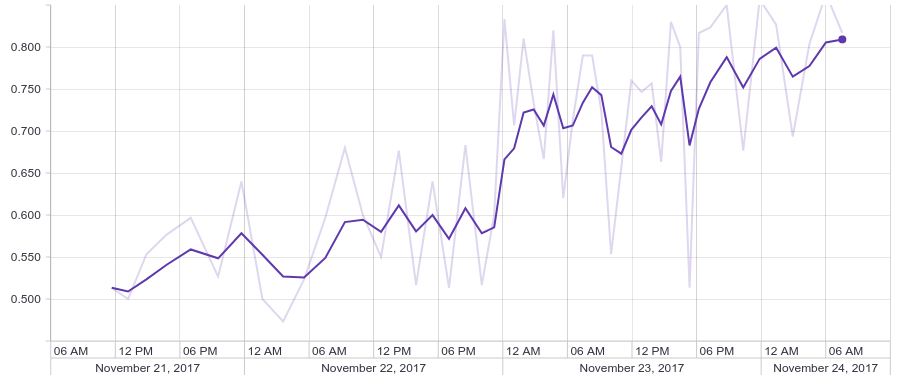
\includegraphics[scale=0.5]{validation_process.png}
\end{center}
\caption{Learning process of the network - the graph shows the developement of the accuracy of the network on the validation set. The darker line represents the smoothed values of the lighter line. Since the training is performed on the CPU (GPU can not be utilized since the network was too big.), it takes several days.}
\label{fig:validation}
\end{figure}

\begin{figure}
\begin{center}
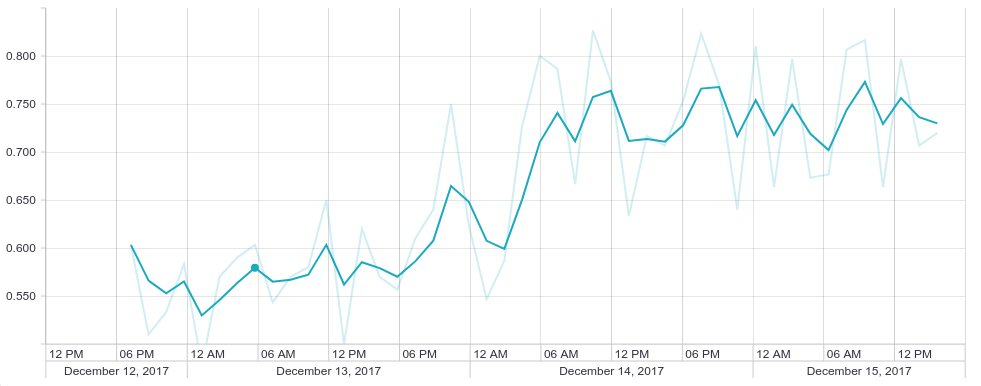
\includegraphics[scale=0.5]{elu_activation.png}
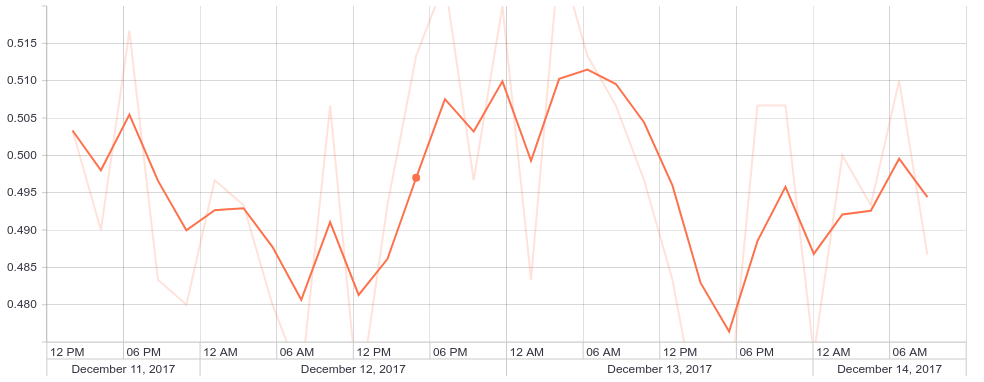
\includegraphics[scale=0.5]{small_batch.png}
\end{center}
\caption{Another activation function in the dense layers (elu) and in the bottom graph with a batch size of 1.}
\label{fig:different_learning}
\end{figure}


\section{Analyzing the Network}
To understand how a network solves the task it makes sense to look at the patterns it's layers a sensitive to. The convolutional layers allow for visual inspection.
Focus on the conv layers, what do they look like? Any hint on the geometry they are sensitive to?
Activation patterns to synthetic data and patches from the patients.

How is that best understood? 2 Approaches: first mean activation of the filters in each layer per img.

\subsection{Mean Class Activation}

\begin{figure}
\begin{center}
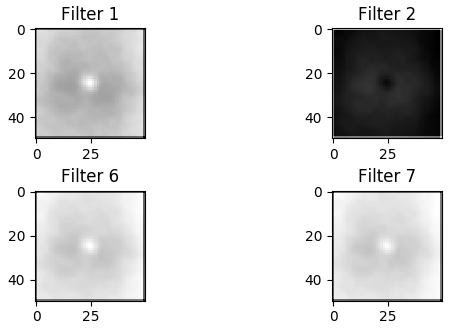
\includegraphics[scale=0.5]{nodule_activation_example.png}
\end{center}
\caption{The mean activation from 500 nodule patches of the validation set. Already in the first layer the receptive field is focusing on the center area, where the nodule resides.}
\label{fig:mean_activation}
\end{figure}


\section{Bridge to other Approaches}
How could a comparison at all be achieved? What is hindering the straightforward comparison of the kernel weights? Draw out a method to do that
Show what has been done
Compare performance to hand crafted approaches, 
take numbers out of papers

what could be similar features in the network?
\end{document}